\documentclass[12pt]{article}
\usepackage{sbc-template}
\usepackage{graphicx,url}
\usepackage{amsmath}
\usepackage{booktabs}
\usepackage{hyperref}
\usepackage{xurl}
\usepackage[utf8]{inputenc}
\usepackage[brazil]{babel}

\sloppy

\title{Previsibilidade dos tempos de viagem da linha 4110 de Belo Horizonte:\\
uma réplica com Modelos Mistos}

\author{João Victor dos Santos\inst{1}\and Felipe Domingos da Cunha\inst{1}}

\address{ICEI -- Pontifícia Universidade Católica de Minas Gerais
  (PUC Minas)\\
  CEP: 30535-901 -- Belo Horizonte -- MG -- Brasil
  \email{1130758@sga.pucminas.br, 342929@sga.pucminas.br}
}

\begin{document}

\maketitle

\begin{abstract}
We replicate, for Belo Horizonte, a mixed-model study of bus travel-time predictability
originally carried out in Curitiba. Using 16 days of GPS positions from bus line 4110
(Belvedere to Dom Cabral, 64 stops) matched to the city's static GTFS feed, we estimated
arrival times at stops for 393 trips and modeled the travel time between consecutive stops.
A random intercept per segment explains 63\% of the variance, and an AR(1) error structure
reduces the out-of-sample error from 62~s (fixed effect only) to 35~s per segment. As an
extension, we compared observed and scheduled times: trips took 70~minutes on average against
53~minutes scheduled, and delay grew by 0.92~minutes per kilometer. The data did not support a
significant afternoon peak effect, mainly because few complete peak-hour trips were recorded.
\end{abstract}

\begin{resumo}
Este trabalho replica, em Belo Horizonte, um estudo sobre a previsibilidade dos tempos de
viagem de ônibus com Modelos Mistos, originalmente realizado em Curitiba. A partir de 16 dias
de posições de GPS da linha 4110 (Belvedere -- Dom Cabral, 64 paradas), cruzadas com o GTFS
estático da cidade, estimou-se o horário de passagem nas paradas em 393 viagens e modelou-se o
tempo de deslocamento entre paradas consecutivas. O intercepto aleatório por trecho explica
63\% da variância, e a estrutura de erro AR(1) reduz o erro fora da amostra de 62~s (apenas
efeito fixo) para 35~s por trecho. Como extensão, compararam-se os tempos observados com os
programados: as viagens duraram em média 70~minutos, contra 53~minutos previstos no quadro de
horários, e o atraso cresceu 0,92~minuto por quilômetro percorrido. Os dados não sustentaram
um efeito significativo do pico da tarde, sobretudo pelo pequeno número de viagens completas
registradas nesse período.
\end{resumo}

\section{Introdução}

O ônibus é o principal meio de transporte coletivo na maior parte das cidades brasileiras, e a
confiabilidade do serviço pesa diretamente na decisão de usá-lo ou não. Quando o passageiro não
consegue prever quanto tempo vai esperar ou quanto vai durar a viagem, ele passa a reservar
mais tempo para cada deslocamento ou migra para outros modos, o que vai na contramão das
políticas de mobilidade de baixo carbono discutidas na literatura \cite{WIMBADI2021103023}.
A percepção de qualidade do transporte público depende, entre outros fatores, da pontualidade e
da regularidade do serviço \cite{https://doi.org/10.1002/atr.106}.

A disponibilidade de dados abertos de geolocalização dos veículos tornou possível medir essa
previsibilidade com frequência e em larga escala. \cite{courb} usaram
dados de GPS dos ônibus de Curitiba e Modelos Mistos para estudar o tempo de deslocamento entre
paradas consecutivas de uma linha, mostrando que a maior parte da variabilidade está associada
ao trecho percorrido e que há dependência temporal entre observações sucessivas. Na mesma
direção, \cite{10.1109/TITS.2022.3145243} tratam a
previsibilidade das operações de transporte como algo que pode ser modelado e acompanhado, e
não apenas como pontualidade.

Este trabalho replica a metodologia de \cite{courb} para Belo Horizonte,
usando como caso de estudo a linha 4110, no sentido Belvedere $\rightarrow$ Dom Cabral. Além
da réplica, o trabalho propõe uma extensão: comparar os horários de passagem observados com o
quadro de horários publicado no GTFS da BHTRANS, para medir o atraso em relação ao programado e
verificar se ele varia com a faixa horária, o tipo de dia e a posição da parada no percurso.

As contribuições do trabalho são: (i) a aplicação da metodologia de Curitiba a outra capital,
com outra fonte de dados, o que permite avaliar a transferibilidade do método; (ii) a
validação fora da amostra dos modelos, com métricas quantitativas; (iii) a medição da
diferença entre o tempo de viagem real e o programado na linha estudada; e (iv) a
disponibilização do código e dos dados utilizados, permitindo a reprodução dos resultados.

O restante do texto está organizado da seguinte forma. A Seção~\ref{sec:relacionados}
apresenta os trabalhos relacionados. A Seção~\ref{sec:metodologia} descreve a coleta, o
tratamento dos dados e os modelos. A Seção~\ref{sec:resultados} apresenta e discute os
resultados, e a Seção~\ref{sec:conclusao} traz as conclusões, as limitações e os trabalhos
futuros.

\section{Trabalhos Relacionados}
\label{sec:relacionados}

\subsection{Propagação de atrasos e confiabilidade do tempo de viagem}

Atrasos em linhas de ônibus raramente são eventos isolados. \cite{Zhang2024} analisam atrasos de chegada em tempo real com um modelo de regressões
aparentemente não relacionadas e mostram que o atraso acumulado nas paradas anteriores é o
fator mais importante para explicar o atraso nas paradas seguintes, enquanto variáveis
meteorológicas têm papel secundário no contexto estudado. Essa ideia de acúmulo ao longo do
percurso é central para a extensão proposta neste trabalho.

Fatores da própria via também afetam a confiabilidade. \cite{KAEWUNRUEN2021100280} investigam as causas da variabilidade do tempo de viagem de
ônibus em Birmingham e apontam características do percurso, como interseções semaforizadas e
o espaçamento entre paradas, entre os elementos que mais pesam. No transporte sobre trilhos,
\cite{doi:10.1177/0361198106195500103} usam
análise computacional e simulação para aumentar a confiabilidade dos horários do S-Bahn de
Zurique, mostrando que o próprio quadro de horários pode ser uma fonte de atraso quando não
reflete os tempos reais de operação.

\subsection{Previsão com dados abertos}

A popularização do padrão GTFS e dos dados de posição em tempo real abriu espaço para modelos
de previsão de atraso. \cite{10857111} comparam modelos de
aprendizado de máquina para prever atrasos a partir de dados GTFS, e
\cite{SARHANI2024100120} discutem como combinar diferentes
fontes de dados abertos para prever atrasos no transporte ferroviário. Sistemas de
rastreamento em tempo real também são apontados como base para melhorar a eficiência da
operação e a informação ao passageiro \cite{10544098}. Esses trabalhos priorizam a acurácia da
previsão; a abordagem adotada aqui prioriza a interpretação, separando a variabilidade que se
deve ao trecho da que se deve à viagem.

\subsection{Modelos Mistos aplicados ao transporte público}

\cite{courb}, trabalho replicado aqui, analisam a linha 863 (Água
Verde) de Curitiba a partir dos dados de GPS publicados pela prefeitura, considerando um
veículo em um itinerário de 18 paradas (17 trechos). A variável resposta é o tempo de
deslocamento entre paradas consecutivas, e o agrupamento é feito pelo trecho. Os autores
comparam um modelo só com efeito fixo, um modelo com intercepto aleatório por trecho e
modelos com erro autorregressivo, incluindo um componente sazonal cujo período é o número de
trechos de uma viagem. O modelo com erro autorregressivo sazonal teve o melhor ajuste, e a
validação foi feita aplicando o modelo ajustado em uma quarta-feira aos dados da
quarta-feira seguinte.

Modelos Mistos são adequados a esse problema porque as observações têm estrutura hierárquica:
várias viagens passam pelos mesmos trechos, e cada viagem gera várias observações
\cite{pinheiro2000}. Isso permite estimar quanto da variabilidade é explicada pelo trecho e
quanto é residual, além de incorporar correlação temporal entre observações.

Este trabalho se diferencia do original em três pontos: usa outra cidade e outra fonte de
dados (a API de tempo real e o GTFS da BHTRANS); modela todas as viagens de uma linha ao longo
de 16 dias, e não um único veículo em um dia; e avalia os modelos fora da amostra com métricas
de erro, além de propor a extensão com o atraso em relação ao horário programado.

\section{Metodologia}
\label{sec:metodologia}

O trabalho segue a metodologia de \cite{courb}, adaptada aos dados
disponíveis em Belo Horizonte, e acrescenta uma análise do atraso em relação ao horário
programado. O processo tem cinco etapas: coleta, pré-processamento, cálculo dos horários de
passagem nas paradas, réplica dos modelos e extensão. Todo o código está disponível no
repositório do trabalho\footnote{\url{https://github.com/JVDS17/tcc}} e reproduz, a partir dos
dados brutos, todas as tabelas e figuras deste texto.

\subsection{Dados}

\textbf{Posições dos veículos.} As posições de GPS foram coletadas por um programa em Python
que consultou, a cada 20 segundos, o \textit{feed} GTFS-Realtime de posições de veículos
(\textit{VehiclePositions}) do sistema de transporte de Belo Horizonte, entre 30/03/2026 e
19/04/2026. O coletor era executado em sessões de 12 horas e gravava os registros das linhas
monitoradas em uma planilha do Google Sheets. Cada registro contém o instante da consulta, a
linha, o veículo, o identificador da viagem no GTFS (\textit{trip\_id}), o horário de partida
programado, a latitude e a longitude; o campo de velocidade veio sempre zerado e não foi
usado. Foram coletados 105.207 registros da linha 4110, em 16 dias. Houve dias sem coleta (01
a 05/04) e períodos com poucos registros, devidos a instabilidades do \textit{feed}, a falhas
de transmissão dos veículos e aos intervalos entre as sessões de coleta.

\textbf{Quadro de horários e traçado.} Usou-se o GTFS estático da BHTRANS \cite{gtfsbh} na
versão baixada pelo próprio coletor em 19/04/2026 (versão 202604181953), em vigor durante a
coleta. Os 95 \textit{trip\_ids} encontrados na coleta existem nesse GTFS. A escolha da versão
importa: versões posteriores mantêm os mesmos identificadores, mas com horários programados
diferentes em cerca de um terço das paradas. Do GTFS foram extraídos o traçado da linha
(\textit{shapes.txt}), as paradas (\textit{stops.txt}) e os horários programados em cada
parada (\textit{stop\_times.txt}).

\textbf{Recorte.} Todas as viagens registradas pertencem ao sentido Belvedere $\rightarrow$
Dom Cabral, que tem 64 paradas e 19,5~km; o sentido contrário não foi capturado pela coleta.
A análise se restringe, portanto, a esse sentido.

\subsection{Pré-processamento}

\textbf{Viagem real.} O \textit{trip\_id} da BHTRANS identifica um horário de partida do
quadro (por exemplo, a partida das 12h52 em dias úteis) e se repete todos os dias. Por isso,
uma viagem realizada foi definida pela combinação de data, \textit{trip\_id} e veículo, o que
resultou em 995 viagens.

\textbf{Posições repetidas.} Embora a API fosse consultada a cada 20~s, os veículos atualizam
a posição com intervalo mediano de 46~s. Leituras consecutivas do mesmo veículo com a mesma
posição foram tratadas como duplicatas e removidas, restando 41.643 registros.

\subsection{Horário de passagem nas paradas}

O GPS registra posições em instantes discretos, que raramente coincidem com a passagem pela
parada. Para estimar esse instante, cada posição foi projetada sobre o traçado da linha,
obtendo-se a distância percorrida $d$ desde o início do percurso. A busca da projeção foi
limitada a uma janela à frente da posição anterior, evitando associar o ônibus a um trecho
errado em locais onde a rota passa perto de si mesma, e posições a mais de 80~m do traçado
foram descartadas. A distância de cada parada $s$ ao longo da rota, $d_s$, vem do próprio GTFS.

O horário de passagem foi obtido por interpolação linear entre as duas posições consecutivas
$P_i$ e $P_{i+1}$ que envolvem a parada ($d_i \le d_s \le d_{i+1}$):
\begin{equation}
T_s = T_i + (T_{i+1} - T_i)\,\frac{d_s - d_i}{d_{i+1} - d_i}
\end{equation}
Interpolações em que $T_{i+1} - T_i > 180$~s foram descartadas, por indicarem perda de sinal;
esse limite cobre 99\% dos intervalos reais de atualização. Para a primeira parada, usou-se o
instante em que o ônibus se afasta 30~m do terminal, isto é, a partida efetiva.

A API associa \textit{trip\_ids} a muitos fragmentos curtos de trajeto (veículos que aparecem
por poucos minutos). Por isso, mantiveram-se apenas as viagens com horário de passagem
calculado em pelo menos 50\% das paradas. Quando dois veículos apareceram com o mesmo
\textit{trip\_id} no mesmo dia, manteve-se o de maior cobertura. Também foram corrigidas as
viagens rotuladas com o dia de serviço errado na virada da meia-noite. Ao final, restaram 393
viagens e 21.871 horários de passagem, com cobertura média de 87\% das paradas.

\subsection{Réplica: tempo de deslocamento entre paradas}

Seguindo \cite{courb}, a variável resposta é o tempo de deslocamento
$t_{jk}$ no trecho $j$ (da parada $j$ à parada $j+1$) na viagem $k$. Os trechos com menos de
100 observações (a saída do terminal e a chegada final) foram excluídos, restando 60 trechos e
21.372 observações. Foram ajustados quatro modelos:

\begin{itemize}
  \item \textbf{M1}, apenas efeito fixo: $t_{jk} = \beta_0 + \varepsilon_{jk}$;
  \item \textbf{M2}, com intercepto aleatório por trecho:
        $t_{jk} = \beta_0 + b_{j} + \varepsilon_{jk}$, com $b_j \sim N(0, \sigma_b^2)$ e
        $\varepsilon_{jk} \sim N(0, \sigma^2)$;
  \item \textbf{M3}, igual ao M2, mas com erro autorregressivo de primeira ordem dentro de cada
        trecho: $\varepsilon_{jk} = \phi\,\varepsilon_{j,k-1} + \eta_{jk}$, em que $k-1$ é a
        viagem anterior que passou pelo mesmo trecho;
  \item \textbf{M3 sazonal}, em que os resíduos do M3, ordenados cronologicamente, recebem um
        modelo AR(1) com componente sazonal AR(1) de período igual ao número de trechos por
        viagem (60).
\end{itemize}

Os modelos M2 e M3 foram ajustados por máxima verossimilhança com o pacote \texttt{nlme} do R
\cite{pinheiro2000}, e o componente sazonal com o pacote \texttt{forecast}
\cite{hyndman2008}. O código partiu do repositório público de \cite{courb}, com três diferenças: o coeficiente $\phi$ é estimado a partir dos dados, e
não fixado; o componente sazonal é estimado por soma de quadrados condicional, porque a
máxima verossimilhança exata não convergiu em uma série com cerca de 24 mil pontos, período 60
e lacunas; e todas as viagens da linha entram no modelo, e não apenas as de um veículo.

\textbf{Avaliação.} Como no artigo original, compara-se o erro quadrático médio (EQM) no
ajuste. Além disso, os modelos foram avaliados fora da amostra de duas formas: (a) ajuste com
os dados de 30/03 a 12/04 e teste com os de 13 a 19/04; e (b) ajuste com a quarta-feira 08/04
e teste com a quarta-feira 15/04, reproduzindo o desenho do artigo. Em ambas, as previsões do
M3 e do M3 sazonal usam os resíduos já observados (previsão um passo à frente), e são
reportados a raiz do erro quadrático médio (RMSE) e o erro absoluto médio (MAE).

\subsection{Extensão: atraso em relação ao horário programado}

O atraso na parada $j$ da viagem $i$ é a diferença entre o horário de passagem estimado e o
programado no GTFS:
\begin{equation}
A_{ij} = T_{ij} - T^{prog}_{ij}
\end{equation}
Valores positivos indicam atraso. No GTFS da BHTRANS, apenas a primeira parada é ponto de
controle; os horários das demais são estimativas da própria operadora. O atraso nas paradas
intermediárias é, portanto, medido em relação a essa estimativa.

Foram ajustados três modelos lineares mistos com o pacote \texttt{lme4} \cite{bates2015}, por
máxima verossimilhança restrita (REML):

\begin{itemize}
  \item \textbf{E1}: $A_{ij} = \beta_0 + \beta_1\,\mathrm{pico}_i + u_i + \varepsilon_{ij}$,
        com $u_i$ o efeito aleatório da viagem real e $\mathrm{pico}_i = 1$ para partidas
        programadas entre 16h e 19h59 em dias úteis. É a formulação proposta na primeira etapa
        deste trabalho.
  \item \textbf{E1b}: igual ao E1, mas com o efeito aleatório pelo \textit{trip\_id}. Foi
        incluído para mostrar o efeito de agrupar a mesma partida de dias diferentes, como
        havia sido feito na primeira etapa.
  \item \textbf{E2}: $A_{ij} = \beta_0 + \boldsymbol{\beta}_f\,\mathrm{faixa}_i +
        \boldsymbol{\beta}_d\,\mathrm{tipo\_dia}_i + \beta_k\,\mathrm{km}_{j} + u_i + v_j +
        \varepsilon_{ij}$, com faixa horária da partida (até 9h, 9h--16h, 16h--20h e após
        20h), tipo de dia (útil, sábado e domingo), distância da parada ao início do percurso
        (km), efeito aleatório da viagem $u_i$ e da parada $v_j$.
\end{itemize}

Como o número de viagens completas no pico da tarde foi pequeno, os modelos E1 e E2 foram
reajustados com um critério de cobertura menos rígido (25\% das paradas) para verificar a
sensibilidade do efeito do pico a esse critério.

\section{Resultados e Discussão}
\label{sec:resultados}

\subsection{Dados analisados}

A Tabela~\ref{tab:dados} resume os dados em cada etapa do tratamento. A perda mais
importante ocorre no filtro de cobertura: das 995 viagens com algum registro de GPS, só 431
tinham horário de passagem calculado em pelo menos metade das paradas. A Tabela~\ref{tab:faixas}
mostra que as viagens analisadas se concentram no entrepico de dias úteis; há apenas 7 viagens
de dias úteis com partida entre 16h e 20h, porque a API devolveu poucos registros nesse
período.

\begin{table}[htbp]
\centering
\caption{Volume de dados em cada etapa.}
\label{tab:dados}
\begin{tabular}{lr}
\toprule
Etapa & Quantidade \\
\midrule
Registros brutos de GPS & 105.207 \\
Registros após remover posições repetidas & 41.643 \\
Viagens reais (data + \textit{trip\_id} + veículo) & 995 \\
Viagens com passagem em $\geq$ 50\% das paradas & 431 \\
Viagens na análise (sem duplicatas) & 393 \\
Horários de passagem estimados & 21.871 \\
Trechos usados na réplica (60 trechos) & 21.372 \\
\bottomrule
\end{tabular}
\end{table}

\begin{table}[htbp]
\centering
\caption{Viagens analisadas por tipo de dia e faixa horária da partida programada.}
\label{tab:faixas}
\begin{tabular}{lrrrr}
\toprule
Tipo de dia & Até 9h & 9h--16h & 16h--20h & Após 20h \\
\midrule
Dia útil & 15 & 300 & 7 & 18 \\
Sábado & 2 & 24 & 8 & 8 \\
Domingo & 1 & 5 & 0 & 5 \\
\bottomrule
\end{tabular}
\end{table}

\subsection{Réplica: tempo de deslocamento entre paradas}

A Tabela~\ref{tab:replica} compara o EQM dos modelos com os valores obtidos por
\cite{courb} em Curitiba. A ordem de grandeza e o padrão de melhora são
semelhantes: o maior ganho vem da inclusão do efeito aleatório do trecho (M1 $\rightarrow$
M2), que reduz o EQM em 63\%, e a estrutura AR(1) traz uma redução adicional de 15\%.

\begin{table}[htbp]
\centering
\caption{Erro quadrático médio no ajuste (s$^2$): linha 4110 de Belo Horizonte e linha 863 de
Curitiba \cite{courb}.}
\label{tab:replica}
\begin{tabular}{lrr}
\toprule
Modelo & BH -- linha 4110 & Curitiba -- linha 863 \\
\midrule
M1 -- efeito fixo & 3.688 & 3.420 \\
M2 -- intercepto aleatório por trecho & 1.352 & 969 \\
M3 -- erro AR(1) & 1.150 & 881 \\
M3 sazonal & 1.316 & 851 \\
\bottomrule
\end{tabular}
\end{table}

O intercepto fixo do M2 é de 72,2~s por trecho, com desvio padrão entre trechos de 48,1~s e
desvio padrão residual de 36,8~s. O trecho explica, portanto, 63\% da variância do tempo de
deslocamento (correlação intraclasse). A Figura~\ref{fig:trechos} mostra o tempo previsto para
cada trecho. Os mais lentos estão no início do percurso, entre a Av. Luiz Paulo Franco e a
Av. Raja Gabaglia, passando pela BR-356 (trechos 4 a 6, cada um com cerca de 3,5~minutos), e
na região central, entre a Rua dos Tupis e a Rua Padre Eustáquio (trecho 34, 3,2~minutos). Os
mais rápidos são trechos curtos entre paradas próximas na mesma avenida, com menos de 25~s.

\begin{figure}[htbp]
  \centering
  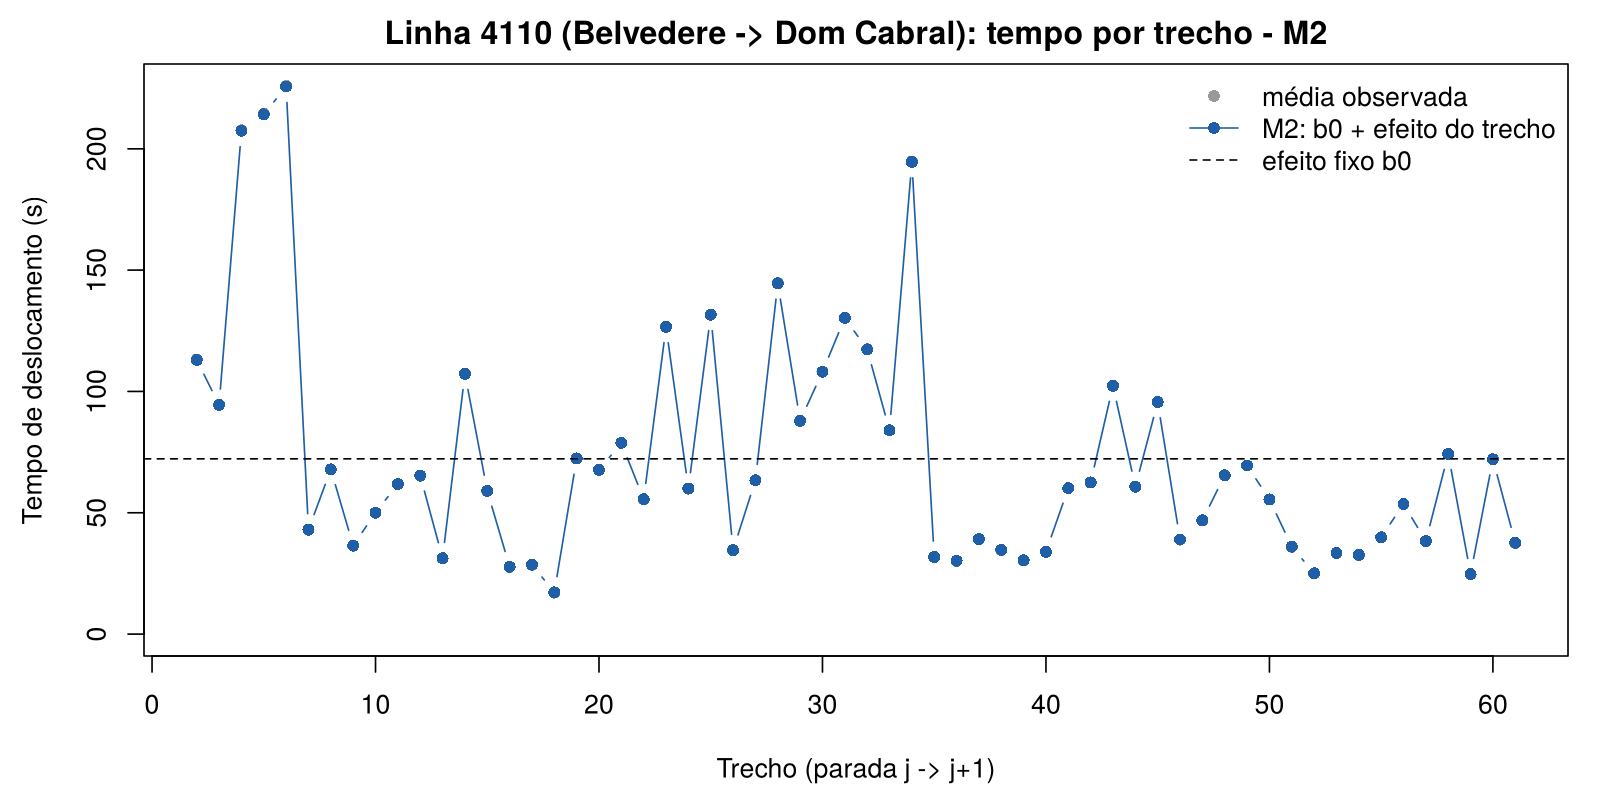
\includegraphics[width=\textwidth]{img/pasquim_efeitos_trecho.png}
  \caption{Tempo de deslocamento médio observado e previsto pelo M2 em cada trecho da linha
  4110 (sentido Belvedere $\rightarrow$ Dom Cabral). A linha tracejada é o efeito fixo
  $\beta_0$.}
  \label{fig:trechos}
\end{figure}

O coeficiente autorregressivo do M3 foi $\phi = 0{,}39$: quando uma viagem é mais lenta que o
esperado em um trecho, a viagem seguinte tende a ser mais lenta no mesmo trecho. A
Figura~\ref{fig:acf} mostra a autocorrelação dos resíduos. No M2 há picos próximos de 60
defasagens, que correspondem ao mesmo trecho na viagem seguinte; esses picos desaparecem no M3
sazonal, cujo componente sazonal estimado foi de 0,43. Ainda assim, o teste de Ljung-Box
indicou autocorrelação residual (p~$<$~0,001), embora pequena em magnitude.

\begin{figure}[htbp]
  \centering
  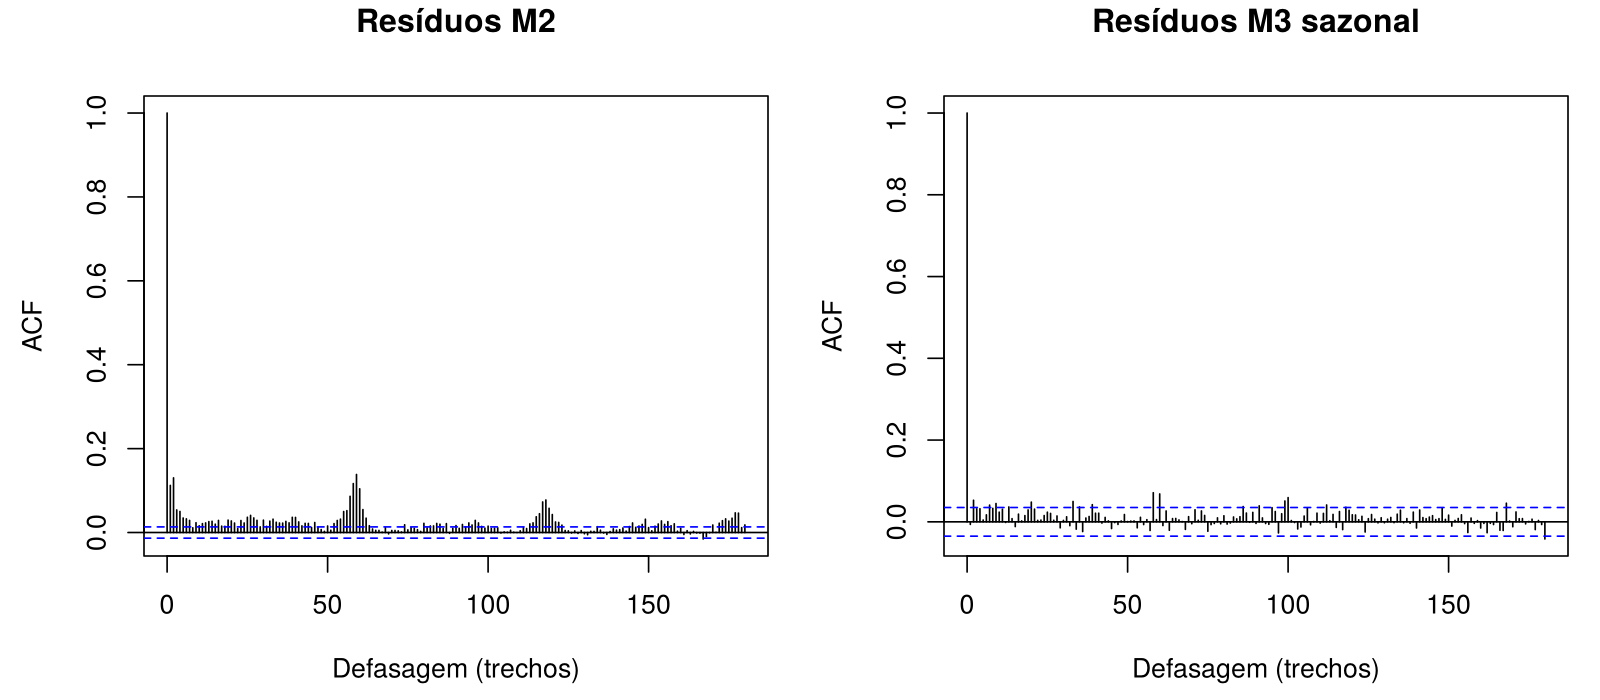
\includegraphics[width=\textwidth]{img/pasquim_acf_residuos.png}
  \caption{Função de autocorrelação dos resíduos do M2 e do M3 sazonal, com defasagem medida
  em trechos.}
  \label{fig:acf}
\end{figure}

Diferentemente de Curitiba, o M3 sazonal não teve o menor EQM. Uma explicação é que, ao
modelar todas as viagens da linha em ordem cronológica, a defasagem sazonal (mesmo trecho,
viagem anterior) coincide com a dependência que o M3 já captura pelo AR(1) dentro do trecho.
No estudo original, com um único veículo, as duas estruturas carregam informações mais
distintas.

A Tabela~\ref{tab:validacao} apresenta a avaliação fora da amostra. Nas duas formas de
validação, o M3 teve o menor RMSE, e o erro típico por trecho caiu de cerca de 60~s no M1 para
cerca de 34~s no M3. O M3 sazonal teve desempenho praticamente igual ao M3. No M2, 95\% das
observações de teste ficaram dentro do intervalo de $\pm 1{,}96\,\sigma$, o que indica que a
variância estimada é adequada. A validação entre quartas-feiras dá resultados próximos aos da
validação com a semana inteira, o que sugere que o padrão por trecho é estável entre as
semanas observadas.

\begin{table}[htbp]
\centering
\caption{Avaliação fora da amostra (erro por trecho, em segundos).}
\label{tab:validacao}
\begin{tabular}{lrrrr}
\toprule
& \multicolumn{2}{c}{Treino 30/03--12/04, teste 13--19/04} & \multicolumn{2}{c}{Treino 08/04, teste 15/04} \\
Modelo & RMSE & MAE & RMSE & MAE \\
\midrule
M1 & 61,8 & 42,7 & 60,0 & 43,1 \\
M2 & 38,6 & 23,0 & 35,5 & 22,3 \\
M3 & 34,8 & 22,1 & 33,7 & 21,6 \\
M3 sazonal & 35,0 & 21,9 & 34,4 & 21,8 \\
\midrule
Observações de teste & \multicolumn{2}{c}{9.556} & \multicolumn{2}{c}{1.787} \\
\bottomrule
\end{tabular}
\end{table}

\subsection{Extensão: atraso em relação ao horário programado}

Nas 258 viagens com registro do início ao fim do percurso, o tempo de viagem observado foi de
69,6~minutos em média (desvio padrão de 7,1), contra 53,1~minutos no quadro de horários. O
atraso médio é de 3,8~minutos na primeira parada com registro e chega a 20,7~minutos na última,
e 85\% dos horários de passagem estão mais de 5~minutos atrasados. A
Figura~\ref{fig:percurso} mostra que o atraso cresce ao longo do percurso, com saltos nos
trechos lentos identificados na réplica: no início (BR-356) e entre os km 7,5 e 11, na
chegada ao centro pela Av. Álvares Cabral e pela Rua São Paulo.

\begin{figure}[htbp]
  \centering
  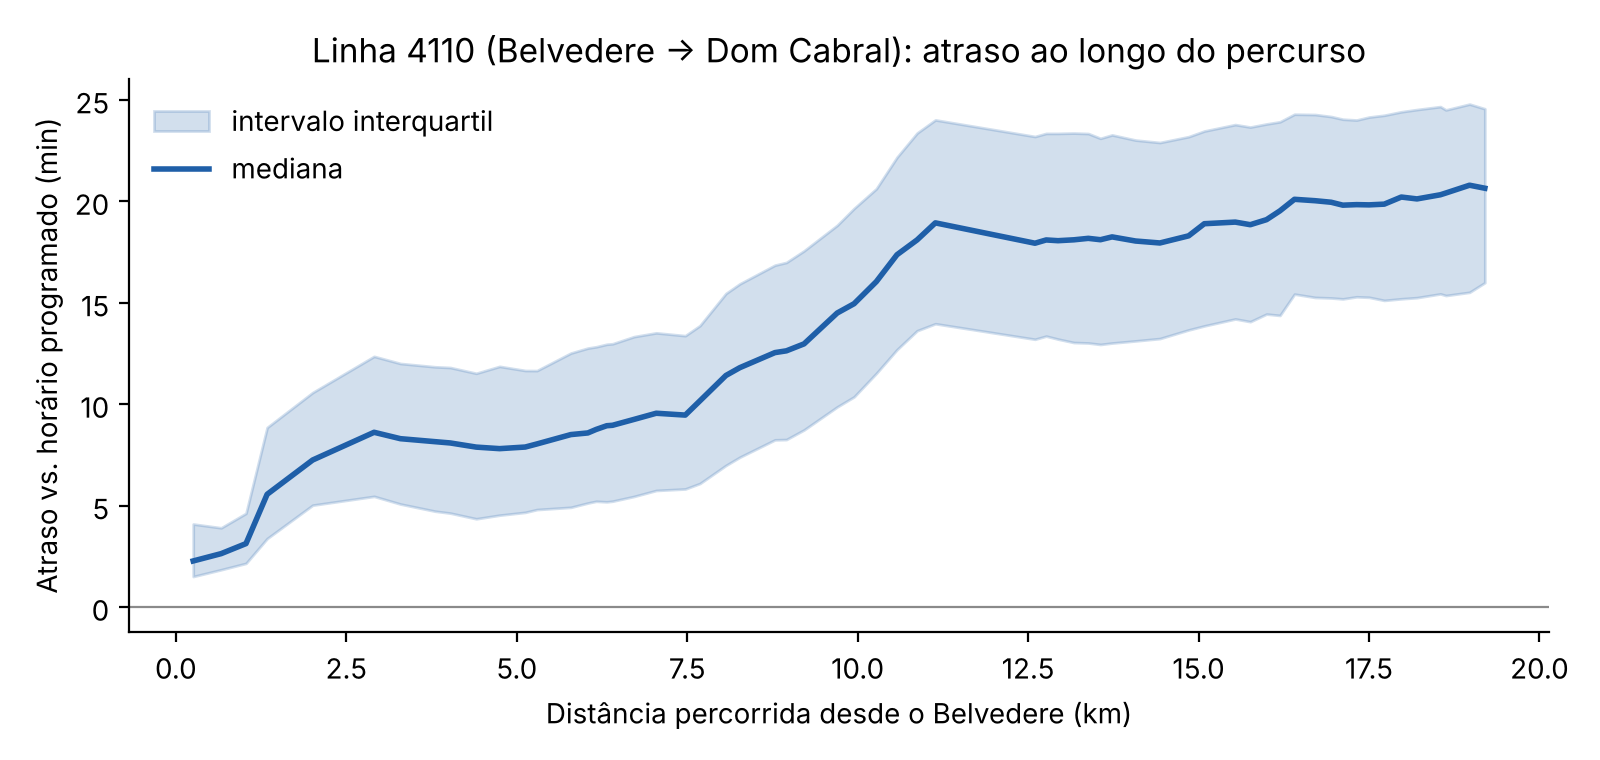
\includegraphics[width=\textwidth]{img/atraso_ao_longo_percurso.png}
  \caption{Atraso em relação ao horário programado ao longo do percurso (mediana e intervalo
  interquartil por parada).}
  \label{fig:percurso}
\end{figure}

A Tabela~\ref{tab:atraso} apresenta os modelos do atraso. No modelo E2, cada quilômetro
percorrido acrescenta 0,92~minuto de atraso (IC95\%: 0,86 a 0,98), controlando a faixa horária
e o tipo de dia. Aos domingos o atraso é 11,3~minutos menor que em dias úteis; aos sábados a
diferença não é significativa. Em relação às partidas até 9h, o atraso é 5,2~minutos menor à
noite, e a diferença no entrepico ($-$2,3~minutos) não é significativa. O efeito aleatório da
viagem (desvio padrão de 5,4~minutos) é bem maior que o da parada (1,3~minuto), uma vez controlada a distância: a maior
parte da diferença entre viagens não é explicada pelas variáveis observadas.

\begin{table}[htbp]
\centering
\caption{Modelos mistos do atraso (minutos). Entre parênteses, intervalo de confiança de 95\%.}
\label{tab:atraso}
\small
\begin{tabular}{lccc}
\toprule
Termo & E1 & E1b & E2 \\
\midrule
Intercepto & 14,2 (13,6; 14,7) & 13,3 (12,0; 14,6) & 7,2 (4,6; 9,8) \\
Pico (16h--20h, dia útil) & 3,1 ($-$1,2; 7,3) & 4,1 ($-$2,9; 11,0) & -- \\
Faixa 9h--16h & -- & -- & $-$2,3 ($-$4,9; 0,2) \\
Faixa 16h--20h & -- & -- & 1,1 ($-$2,7; 4,9) \\
Faixa após 20h & -- & -- & $-$5,2 ($-$8,4; $-$2,1) \\
Sábado & -- & -- & $-$0,7 ($-$2,5; 1,2) \\
Domingo & -- & -- & $-$11,3 ($-$14,6; $-$7,9) \\
Distância (por km) & -- & -- & 0,92 (0,86; 0,98) \\
\midrule
DP efeito aleatório & 5,6 (viagem) & 6,0 (\textit{trip\_id}) & 5,4 (viagem); 1,3 (parada) \\
DP residual & 5,6 & 6,9 & 2,6 \\
\bottomrule
\end{tabular}
\end{table}

O efeito do pico da tarde não foi significativo em nenhum modelo. No E1 a estimativa é de
3,1~minutos, com intervalo que inclui o zero, e no E2 o efeito desaparece quando se controla a
distância. Com o critério de cobertura de 25\%, o número de viagens de pico em dias úteis
passa de 7 para 28 e o efeito no E1 sobe para 4,0~minutos (IC95\%: 1,6 a 6,4), mas no E2
continua não significativo (2,6~minutos; IC95\%: $-$0,4 a 5,7). Como as viagens incompletas
tendem a ser observadas só em parte do percurso, o modelo sem a distância confunde a posição
da parada com o efeito do horário. Esses resultados não permitem afirmar que o pico da tarde
aumenta o atraso na linha 4110; permitem apenas dizer que, se esse efeito existe, os dados
coletados são insuficientes para estimá-lo com precisão.

A comparação entre E1 e E1b mostra por que a primeira etapa deste trabalho havia encontrado
um efeito do pico maior: ao agrupar pelo \textit{trip\_id}, viagens de dias diferentes são
tratadas como se fossem a mesma, o que reduz o número de grupos de 393 para 85 e altera tanto
o intercepto quanto o efeito estimado do pico.

\subsection{Comparação entre semanas}

A Tabela~\ref{tab:semanas} compara o atraso médio por viagem em cada dia da semana nas duas
semanas completas de coleta. As diferenças são pequenas (no máximo 0,8~minuto) e não há
tendência de piora na segunda semana. O padrão se repete nas duas: atrasos de 15 a 17~minutos
de terça a sexta, de 13 a 14~minutos no sábado, cerca de 12~minutos na segunda-feira e de 2 a
3~minutos no domingo. A
Figura~\ref{fig:hora} mostra o atraso médio por hora de partida nos dias úteis: as duas
semanas praticamente coincidem entre 10h e 16h, onde há mais viagens, e se afastam nas horas
com poucas viagens, em que a média é instável.

\begin{table}[htbp]
\centering
\caption{Atraso médio por viagem (minutos) e número de viagens em cada dia da semana.}
\label{tab:semanas}
\begin{tabular}{lrrrrr}
\toprule
& \multicolumn{2}{c}{Semana 1 (06--12/04)} & \multicolumn{2}{c}{Semana 2 (13--19/04)} & \\
Dia & Atraso & Viagens & Atraso & Viagens & Diferença \\
\midrule
Segunda & 11,4 & 35 & 11,9 & 36 & 0,5 \\
Terça & 15,3 & 34 & 15,2 & 24 & $-$0,1 \\
Quarta & 15,8 & 29 & 15,0 & 33 & $-$0,8 \\
Quinta & 16,1 & 15 & 15,6 & 32 & $-$0,5 \\
Sexta & 16,8 & 15 & 16,7 & 28 & $-$0,1 \\
Sábado & 14,1 & 26 & 13,3 & 16 & $-$0,8 \\
Domingo & 2,5 & 5 & 2,3 & 6 & $-$0,2 \\
\bottomrule
\end{tabular}
\end{table}

\begin{figure}[htbp]
  \centering
  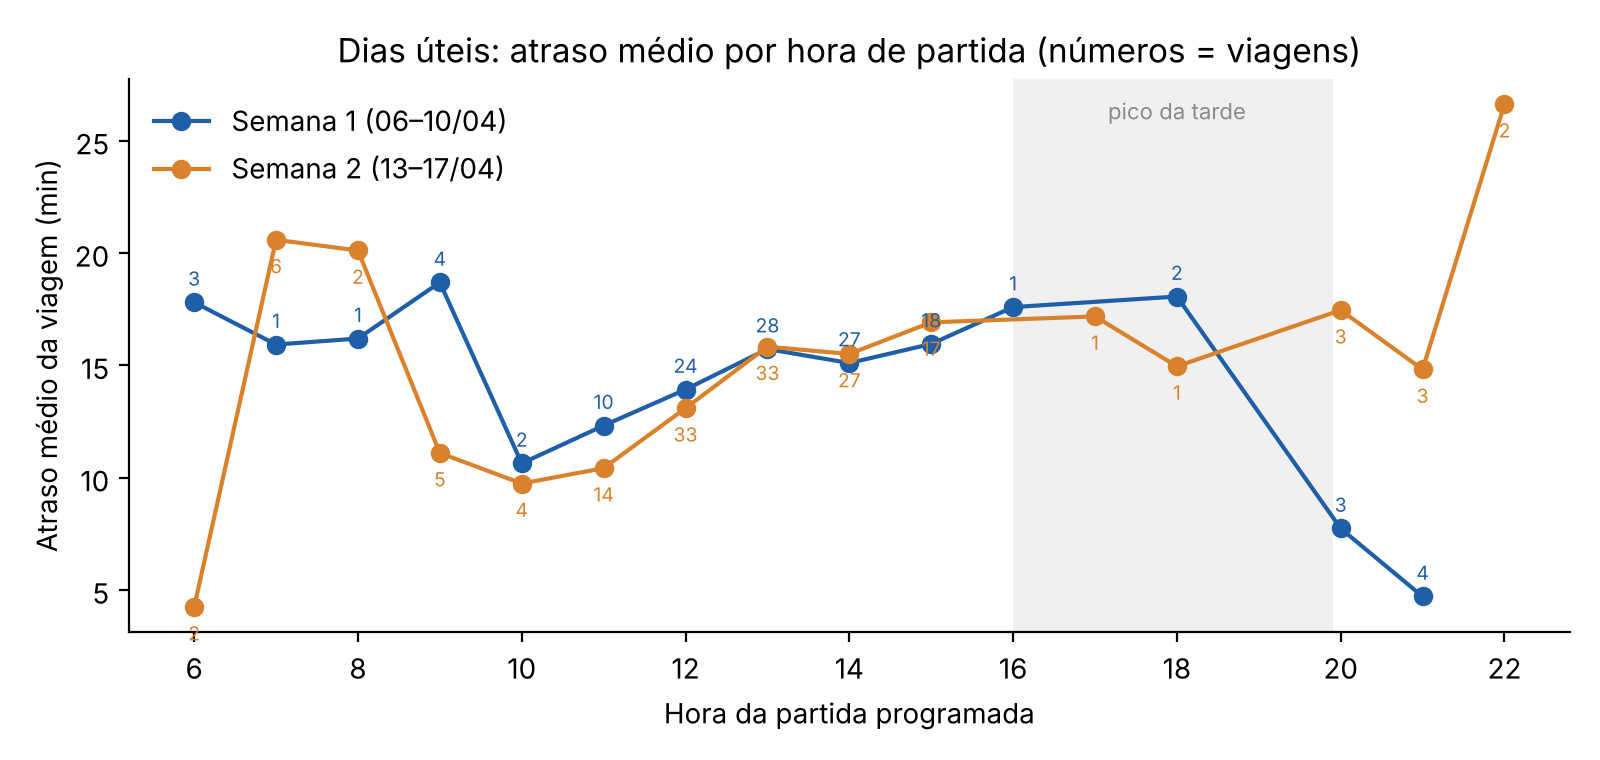
\includegraphics[width=\textwidth]{img/atraso_por_hora_semanas.png}
  \caption{Atraso médio por hora de partida programada em dias úteis, nas duas semanas. Os
  números indicam a quantidade de viagens em cada ponto.}
  \label{fig:hora}
\end{figure}

\subsection{Discussão}

Os resultados reproduzem o principal achado de \cite{courb}: o trecho
é a maior fonte de variabilidade do tempo de deslocamento, e existe dependência entre viagens
sucessivas. Isso indica que a metodologia é transferível entre cidades e fontes de dados, desde
que as diferenças de formato sejam tratadas, como a reutilização dos \textit{trip\_ids} e a
frequência real de atualização do GPS. A estabilidade dos modelos entre semanas reforça que o
padrão por trecho é estrutural.

A extensão mostra que a linha opera, de forma sistemática, com tempo de viagem cerca de 30\%
maior que o programado. O crescimento do atraso ao longo do percurso é compatível com o
acúmulo de atrasos descrito por \cite{Zhang2024} e com a observação
de \cite{doi:10.1177/0361198106195500103} de
que um quadro de horários que não reflete a operação real é, ele mesmo, uma fonte de atraso.
Como os horários intermediários do GTFS são estimativas, parte do atraso medido pode vir dessa
estimativa e não da operação. Ainda assim, a diferença de 16,5~minutos no tempo total da viagem
não depende dos horários intermediários, e sugere que o quadro de horários da linha poderia ser
revisto, sobretudo nos trechos lentos identificados pela réplica.

\section{Conclusão}
\label{sec:conclusao}

Este trabalho replicou, para a linha 4110 de Belo Horizonte, a análise de previsibilidade de
tempos de deslocamento com Modelos Mistos proposta por \cite{courb} para
Curitiba. Com 393 viagens observadas em 16 dias, o intercepto aleatório por trecho explicou
63\% da variância, e o modelo com erro AR(1) reduziu o erro de previsão fora da amostra de
62~s para 35~s por trecho. O padrão foi estável entre as duas semanas analisadas, o que indica
que a metodologia é transferível para outra cidade e outra fonte de dados.

A extensão proposta mostrou que as viagens duraram em média 70~minutos, contra 53~minutos no
quadro de horários, e que o atraso cresce 0,92~minuto por quilômetro percorrido. Os trechos
mais lentos, na região da BR-356 e no centro, concentram boa parte desse acúmulo. Esses
resultados podem subsidiar a revisão do quadro de horários da linha e a priorização de
intervenções nos trechos críticos. Por outro lado, os dados não permitiram estimar com
precisão o efeito do pico da tarde, e não foi observada piora entre as semanas.

\subsection{Limitações}

\begin{itemize}
  \item A coleta capturou apenas o sentido Belvedere $\rightarrow$ Dom Cabral; os resultados
        não podem ser estendidos ao sentido contrário.
  \item Foram 16 dias de coleta, com lacunas, e poucas viagens completas no início da manhã,
        no pico da tarde e aos domingos.
  \item Mais da metade das viagens com registro foi descartada por cobertura insuficiente,
        o que pode introduzir viés se as viagens descartadas tiverem comportamento diferente.
  \item Os horários programados nas paradas intermediárias são estimativas do GTFS, e não
        horários fiscalizados.
  \item O atraso é medido em relação ao \textit{trip\_id} informado pela API; se um veículo
        for rotulado com a viagem errada, o atraso dessa viagem fica distorcido. Os tempos de
        deslocamento entre paradas, usados na réplica, não dependem desse rótulo.
\end{itemize}

\subsection{Trabalhos futuros}

\begin{itemize}
  \item Coletar os dois sentidos da linha por um período mais longo, com monitoramento da
        coleta para reduzir as lacunas, sobretudo no pico.
  \item Incluir variáveis explicativas nos modelos, como chuva, distância e número de
        semáforos de cada trecho, e testar inclinações aleatórias por faixa horária.
  \item Aplicar a metodologia a outras linhas de Belo Horizonte, incluindo linhas do MOVE, e
        comparar a previsibilidade entre corredores.
  \item Usar os modelos para gerar previsões de chegada em tempo real e compará-las com as
        previsões disponibilizadas aos passageiros.
\end{itemize}


\bibliographystyle{sbc}
\bibliography{sbc-template}

\end{document}
